

\tikzset{every picture/.style={line width=0.75pt}} %set default line width to 0.75pt        

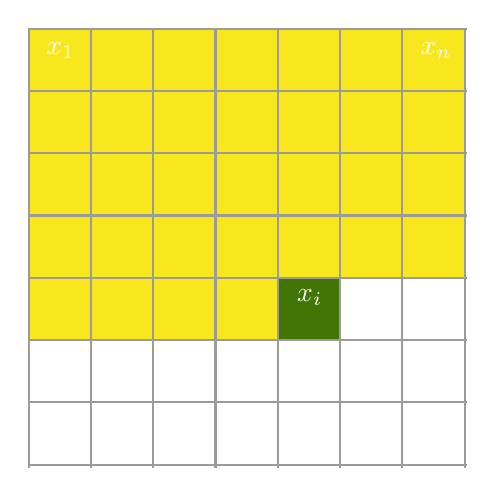
\begin{tikzpicture}[x=0.75pt,y=0.75pt,yscale=-1,xscale=1]
%uncomment if require: \path (0,300); %set diagram left start at 0, and has height of 300

%Shape: Rectangle [id:dp15192004475831844] 
\draw  [draw opacity=0][fill={rgb, 255:red, 65; green, 117; blue, 5 }  ,fill opacity=1 ] (500,160.5) -- (530,160.5) -- (530,190.5) -- (500,190.5) -- cycle ;
%Shape: Rectangle [id:dp01470597311147892] 
\draw  [color={rgb, 255:red, 113; green, 151; blue, 224 }  ,draw opacity=1 ][fill={rgb, 255:red, 248; green, 231; blue, 28 }  ,fill opacity=1 ] (380,160.5) -- (500.14,160.5) -- (500.14,190.5) -- (380,190.5) -- cycle ;
%Shape: Rectangle [id:dp02334866211052944] 
\draw  [color={rgb, 255:red, 113; green, 151; blue, 224 }  ,draw opacity=1 ][fill={rgb, 255:red, 248; green, 231; blue, 28 }  ,fill opacity=1 ] (380,40.5) -- (590,40.5) -- (590,160.5) -- (380,160.5) -- cycle ;
%Shape: Grid [id:dp0019256500858937375] 
\draw  [draw opacity=0] (380,40.5) -- (591,40.5) -- (591,252) -- (380,252) -- cycle ; \draw  [color={rgb, 255:red, 155; green, 155; blue, 155 }  ,draw opacity=1 ] (380,40.5) -- (380,252)(410,40.5) -- (410,252)(440,40.5) -- (440,252)(470,40.5) -- (470,252)(500,40.5) -- (500,252)(530,40.5) -- (530,252)(560,40.5) -- (560,252)(590,40.5) -- (590,252) ; \draw  [color={rgb, 255:red, 155; green, 155; blue, 155 }  ,draw opacity=1 ] (380,40.5) -- (591,40.5)(380,70.5) -- (591,70.5)(380,100.5) -- (591,100.5)(380,130.5) -- (591,130.5)(380,160.5) -- (591,160.5)(380,190.5) -- (591,190.5)(380,220.5) -- (591,220.5)(380,250.5) -- (591,250.5) ; \draw  [color={rgb, 255:red, 155; green, 155; blue, 155 }  ,draw opacity=1 ]  ;

% Text Node
\draw (387,45.65) node [anchor=north west][inner sep=0.75pt]  [color={rgb, 255:red, 255; green, 255; blue, 255 }  ,opacity=1 ]  {$x_{1}$};
% Text Node
\draw (567.29,45.65) node [anchor=north west][inner sep=0.75pt]  [color={rgb, 255:red, 255; green, 255; blue, 255 }  ,opacity=1 ]  {$x_{n}$};
% Text Node
\draw (507.86,164.51) node [anchor=north west][inner sep=0.75pt]  [color={rgb, 255:red, 255; green, 255; blue, 255 }  ,opacity=1 ]  {$x_{i}$};
% Text Node
\draw (566.14,222.51) node [anchor=north west][inner sep=0.75pt]  [color={rgb, 255:red, 255; green, 255; blue, 255 }  ,opacity=1 ]  {$x_{n^{2}}$};


\end{tikzpicture}
